\documentclass[12pt]{report}
\usepackage[utf8]{inputenc}
\usepackage[T1]{fontenc}
\usepackage[portuguese, brazil, english]{babel}
\usepackage{graphics}
\usepackage{url}
\usepackage{lipsum}
\usepackage{graphicx}
\usepackage{geometry}
\usepackage{amssymb}
\usepackage{float}
\usepackage{verbatim} 
\usepackage{amsmath} 
\usepackage{amsfonts}
\usepackage{amssymb}
\usepackage{lmodern}
\usepackage[portuguese,ruled,lined]{algorithm2e}
\usepackage{algorithmic}
\usepackage{caption}
\usepackage{subcaption}
\usepackage{indentfirst}
\usepackage{mathrsfs,amsmath}
\usepackage{amstext}
\usepackage{hyperref}
\usepackage{setspace}
\usepackage[refpage]{nomencl}
\usepackage{nomencl}
% \usepackage[alf,abnt-etal-cite=2,abnt-etal-list=0,abnt-etal-text=it,versalete,bibjustif]{abntex2cite}
\usepackage[alf]{abntex2cite}

\usepackage{epstopdf}
\usepackage{datetime}
%\usepackage[acronym]{glossaries}
%\usepackage{glossaries}
\usepackage{acro}
%\usepackage[acronym]{glossaries}
%\usepackage{longtable}
% probably a good idea for the nomenclature entries:
%\acsetup{first-style=short}
% class `abbrev': abbreviations:
%\DeclareAcronym{ny}{
%  short = NY ,
%  long  = New York ,
%  class = abbrev
%}
%\DeclareAcronym{la}{
%  short = LA ,
%  long  = Los Angeles ,
%  class = abbrev
%}
%\enableregime[utf]

\hypersetup{
    %bookmarks=true,         % show bookmarks bar?
    unicode=false,          % non-Latin characters in Acrobat’s bookmarks
    pdftoolbar=true,        % show Acrobat’s toolbar?
    pdfmenubar=true,        % show Acrobat’s menu?
    pdffitwindow=false,     % window fit to page when opened
    pdfstartview={FitH},    % fits the width of the page to the window
    pdftitle={My title},    % title
    pdfauthor={Author},     % author
    pdfsubject={Subject},   % subject of the document
    pdfcreator={Creator},   % creator of the document
    pdfproducer={Producer}, % producer of the document
    pdfkeywords={keyword1, key2, key3}, % list of keywords
    pdfnewwindow=true,      % links in new PDF window
    colorlinks=true,       % false: boxed links; true: colored links
    linkcolor=blue,          % color of internal links (change box color with linkbordercolor)
    citecolor=blue,        % color of links to bibliography
    filecolor=magenta,      % color of file links
    urlcolor=blue           % color of external links
}
\geometry{left=2.5cm, top=2cm, bottom=2.5cm, right=2cm}
\newcommand{\euler}{\textit{e}}
\newcommand{\complexSymbol}{\textit{j}}
\setstretch{1.5}

\hfuzz=30pt
%\vfuzz=20pt
\hbadness=2000
\vbadness=\maxdimen

\def\worktitle{Desenvolvimento de um {\it drum pad} usando visão artificial}
\def\workauthor{Luciano Rodrigues Lucio Neto}
\def\workadvisor{Agostinho de Medeiros Brito Júnior}

\usepackage{afterpage}

\newcommand\blankpage{%
    \null
    \thispagestyle{empty}%
    \addtocounter{page}{-1}%
    \newpage}


\acsetup{first-style=short}

% Exemplos de acrônimos, se necessários...
% class `abbrev': abbreviations:
\DeclareAcronym{DFT}{
  short = DFT ,
  long  = \textit{Discrete Fourier Transform} ,
  class = abbrev
}
\DeclareAcronym{IDFT}{
  short = IDFT ,
  long  = \textit{Inverse Fourier Transform} ,
  class = abbrev
}
\DeclareAcronym{FFT}{
  short = FFT ,
  long  = \textit{Fast Fourier Transform} ,
  class = abbrev
}

\DeclareAcronym{IFFT}{
  short = IFFT ,
  long  = \textit{Inverse Fast Fourier Transform} ,
  class = abbrev
}
\DeclareAcronym{2D DFT}{
  short = 2D DFT ,
  long  = \textit{Two-Dimensional Discrete Fourier Transform} ,
  class = abbrev
}

\providecommand{\keywords}[1]{\textbf{\textit{Keywords: }} #1}
\providecommand{\palavrasChaves}[1]{\textbf{\textit{Palavras-chaves: }} #1}

\newdateformat{monthyeardate}{%
  \monthname[\THEMONTH], \THEYEAR}
%%%%%%%%%%%%%%%%%%%%%%%%%%%%%%%%%%%%%%%%%%%%%%%%%%%%%%%%%%%%%
\begin{document}

\selectlanguage{brazil}
\begin{titlepage}

	\centering
	{\normalsize \workauthor \par}
	%\includegraphics[width=0.15\textwidth]{example-image-1x1}\par\vspace{1cm}
	%{\scshape\LARGE Universidade Federal do Rio Grande do Norte \par}
	\vfill
	{\Large\bfseries \worktitle \par}
	\vfill

% Bottom of the page

	{\normalsize Brasil\par}
	{\normalsize \monthyeardate\today}
\end{titlepage}

\begin{titlepage}

	\centering
	{\normalsize \workauthor\par}
	%\includegraphics[width=0.15\textwidth]{example-image-1x1}\par\vspace{1cm}
	%{\scshape\LARGE Universidade Federal do Rio Grande do Norte \par}
	\vfill
	\centering
	{\Large\bfseries \par}
	\vfill

	\begin{flushright}	
	\begin{minipage}{15em}	
	\setstretch{1.0}
  	Trabalho de Conclusão de Curso Submetido à Coordenação do Curso de Engenharia de Computação e Automação do Centro de Tecnologia da Universidade Federal do Rio Grande do Norte, como parte dos requisitos necessários para a obtenção do grau de Engenheiro de Computação.
	\end{minipage}
	\end{flushright}	
	\vfill
	
	
	{\small Universidade Federal do Rio Grande do Norte - UFRN \par}
	{\small Coordenação do Curso de Engenharia de Computação e Automação - DCA \par}
	{\small Graduação em Engenharia de Computação \par}
	\vfill
	\normalsize
	\centering
	{\normalsize Orientador: Agostinho de Medeiros Brito Júnior \par}
	\vfill
% Bottom of the page
	{\normalsize Brasil\par}
	{\normalsize \monthyeardate\today}
\end{titlepage}

\pagenumbering{gobble}% Remove page numbers (and reset to 1)

%%%%%% AGRADECIMENTOS %%%%%%

\begin{center}
%{\bf \Large Agradecimentos}
\end{center}
%Gostaria de agradecer a...

\newpage

%%%%%% RESUMO %%%%%%

\begin{abstract}
  Apresenta o desenvolvimento de um {\it drum pad} usando visão
  artificial capaz de controlar sintetizadores musicais criando uma
  sequência de notas musicais em repetição. Instrumentos assim são
  muito usados por músicos amadores que precisam criar acompanhamentos
  de bateria ou baixo para suas composições e não dispõem de músicos
  auxiliares para fazê-lo. A ferramenta criada permite que, usando
  apenas uma webcam, uma folha de papel e software livre, um músico
  amador seja capaz de criar efeitos semelhantes aos de um drum pad
  físico desenhando ou sobrepondo pequenas fichas coloridas na folha
  de papel.
  \\
  \palavrasChaves{Drum pad, sequenciador, controlador midi, OpenCV,
    Visão artificial}
\end{abstract}

\newpage

%%%%%% RESUMO EM INGLÊS %%%%%%
\selectlanguage{english}

\begin{abstract}
  abstract in english
  \\
  \keywords{translate-as}

\end{abstract}

\newpage

\selectlanguage{brazil}

%%%%%% LISTA DE FIGURAS %%%%%%

\listoffigures

\newpage

%%%%%% LISTA DE ABREVIAÇÕES %%%%%%

%{\centering
%\printacronyms[include-classes=abbrev,name=Abreviações]
%}
\tableofcontents

%\makenomenclature
%\makeglossaries

%\newglossaryentry{DFT}{%
%name={DFT},%
%description={antigeen-presenterende cel}%
%}


\newpage

%%%%%% INÍCIO DO TEXTO %%%%%%

\pagenumbering{arabic}

\chapter{Introdução}
\label{cha:introducao}

Um {\it drum pad} é um periférico utilizados por diferentes segmentos da sociedade de diferentes formas. Sua principal função é reproduzir sons escolhidos pelo usuário ao apertar de botões de sua interface e, por isso, é comumente utilizado principalmente pela comunidade de músicos sendo eles profissionais ou amadores.
Utilizado também como uma forma de se programar uma sequência de sons que será reproduzida em um intervalo de tempo específico, um {\it drum pad} serve como acompanhamento musical com diversas aplicações sejam elas para guiar um músico, acompanhar o ritmo com alguma percussão ou até reproduzir detalhes específicos que o usuário pode não conseguir no momento correto.

Apesar de ser um periférico de fácil utilização e de rápida adaptabilidade, ainda depende da capacidade do usuário em reproduzir as notas no tempo correto e principalmente da capacidade que o usuário tem em investir num equipamento do tipo, variando de cerca de 50 dólares, podendo chegar a mais de 600 dólares, dependendo do seu tamanho, sua funções, caracterísitcas, inovações e acabamento.

A proposta do projeto apresentado neste trabalho de conclusão de curso é de facilitar a programação de uma sequência de sons que um usuário venha querer utilizar para qualquer propósito que seja, principalmente os descritos anteriormente. Com apenas uma webcam de cerca de 60 dólares, uma folha de papel e um programa de computador que utiliza conceitos de visão artificial, o usuário é capaz de programar, de forma interativa, uma sequência de sons provenientes de um sintetizador midi, que será reproduzida em um tempo determinado sem depender, por exemplo, de suas próprias habilidades rítmicas, a partir de marcações feitas na folha.

No capítulo XX serão apresentados..., no capítulo XX será mostrado
... . O capítulo XX discorre sobre.... blá, blá, blá...

\chapter{Modelo para Interpretação}
\label{cha:fund-teor}

Como muitas aplicações que envolvam conceitos de visão artificial, é necessário um ambiente controlado de onde se possa extrair as informações necessárias para o funcionamento do programa de computador. Para isso, foi necessária a criação de um {\it layout} com elementos específicos que façam com que o ambiente seja bem interpretado pelo programa.

IMAGEM DO LAYOUT

As principais características do {\it layout} para que haja a interação com o programa de computador são os  marcadores nos cantos da folha e o código de barras. Tendo em vista que, nesse modelo, sempre haverão 13 notas distintas que podem ser reproduzidas, o código de barras é utilizado para guardar a informação de quantas notas o programa pode reproduzir e sua fórmula de compasso, sem haver a necessidade do usuário especificá-las já que não faria sentido o modelo ter, por exemplo, uma área quadriculada de 13x8 e o usuário configurar que o essa área tem uma distribuição diferente da real ou uma fórmula de compasso que não corresponda ao modelo. Além do código de barras, são utilizados marcadores nos cantos da folha que, ao serem interpretados, mostram a imagem final que o programa utilizará como fonte de interpretação.

\chapter{Algoritmo}
\label{cha:fund-teor}

Partindo da imagem capturada da câmera do usuário, o programa procura os marcadores dos cantos da folha, o código de barras e os interpreta guardando as informações necessárias. Essas verificações acontecem a cada frame capturado pela câmera para manter a integridade com a imagem de tempo real.
Com pontos capturados a partir dos marcadores, é selecionada a área de interesse da folha que o programa deverá interpretar ao sinal do usuário.

IMAGEM DA ÁREA DO MEIO DA FOLHA

Com a informação de quantas colunas existem na área quadriculada, adquirida do código de barras presente na folha, a próxima etapa executada pelo algoritmo é de verficiar, em cada um dos retângulos da área de interesse, se há dois tipos de marcações diferentes: uma representa um som que só tocará naquele momento e a outra representa a continuidade do som, permitindo que ela seja reproduzido durante o tempo desejado pelo usuário. Foram escolhidas duas marcações diferentes para o software identificar quando deve ocorrer cada uma das duas situações. O que identifica se a nota será ou não mantida, é haver ou não pixels marcados do meio da marcação original padrão até o final do quadrado identificado pelo programa.

IMAGEM DA MARCAÇÃO SOZINHA E IMAGEM DA MARCAÇÃO CONTINUADA (LADO A LADO)

A partir das informações que o programa consegue da etapa anterior, ele envia mensagens MIDI, utilizando o protocolo MIDI, para se comunicar com uma fonte de áudio selecionada pelo usuário, a qual será responsável pela reprodução dos sons em sí. Isso tudo com um intervalo de tempo definido entre cada nota, devido à cálculos a partir da fórmula do compasso daquele modelo, extraída do código de barras da folha, e definida ao gerar o pdf a partir de um segundo programa criado para esse propósito.

Os cálculos feitos para se obter o tempo de cada som é um simples cálculos utilizando a fórmula do compasso e o valor de batidas por minuto passado como parâmetro, pelo usuário, ao executar o software:

CALCULO: tempo = 60/bpm, para se obter o número de batidas por segundo uma vez que as funções disponíveis no C++ para cálculo de tempo utilizam segundos. Após isso, o tempo de cada som precisa ser divido pelo denominador da fórmula do compasso, para que, em cada batida, sejam tocadas o número de notas definidos pela fórmula e pela convenção feita no desenvolvimento do software, que é a seguinte: para cada fórmula de compasso apresentada pelo usuário, cada retângulo do modelo da folha representará a metade da metade do tempo de uma nota, menos quando o denominador for o número um. Por exemplo: se o usuário passar uma fórmula de compasso 3/4, que representa que em um compasso haverá três semínimas, o modelo da folha, ao invés de 3 retângulos, uma para cada semínima possível, ou 48 colunas, uma para cada semifusa possível, terá 12 colunas, uma para cada semicolcheia. A partir da convenção e da fórmula do compasso, utilizando uma fórmula 3/4, teremos que, no tempo de cada batida serão reproduzidas 4 notas, ou seja, cada coluna tem um intervalo de tempo de 60/(bpm*denominador_formula)

A ordem de disposição das notas foi escolhida da maneira como mostrada na imagem (REFERENCIA A IMAGEM) pois é o mais próximo de como uma "pista" MIDI é representada em softwares profissionais de gravação de músicas, denominados DAW ({\it Digital Audio Workstation}),quando o usuário utiliza recursos MIDI, como se pode ver na imagem abaixo:

IMAGEM DO REAPER DE UMA MIDI TRACK

Também podemos interpretar o layout como um gráfico num simples plano cartesiano. O gráfico representa frequência \times\ tempo e é digital e discreto, fazendo com que a posição da marcação represente uma frequência num intervalo de tempo. Essa interpretação pode ser representada da seguinte maneira:

IMAGEM DO LAYOUT COM MARCAÇÕES E GRÁFICO LADO A LADO

\chapter{Protocolo MIDI}
\label{cha:fund-teor}

O Protocolo MIDI é o principal responsável pela reprodução dos sons de sintetizadores e sequenciadores MIDI e, sendo um protocolo, é universal, ou seja, independe do fabricante do sintetizador ou sequenciador uma vez seguido de maneira correta. Apesar de bastante extenso e complexo, serão explicadas aqui apenas conceitos que foram utilizados no desenvolvimento do projeto.

Esse protocolo consiste na troca de "mensagens MIDI" entre o software ou hardware controlador, que controla os sons, e do software ou hardware sintetizador, que sintetiza os sons. É utilizado para transmissão de informação em tempo real entre controlador e sintetizador a fim de gerar sons quando o usuário desejar.

Essas mensagens baseam-se em um conjunto de um ou mais {\it bytes}, onde o primeiro {\it byte} se classifica como {\it STATUS byte}, o qual define o tipo da mensagem, e é geralmente seguido por outros {\it bytes} chamados {\it DATA bytes}, os quais dão as características desejadas para a mensagem.

Existem diversos tipos de mensagens, mostradas na tabela (REFERENCIA TABELA) e de forma expandida na tabela (REFERENCIA TABELA), extraídas diretamente da {\it The MIDI Association} (www.midi.org), principal portal com informações do protocolo MIDI, porém, para o desenvolvimento do projeto descrito nesta tese de conclusão de curso, foram utilizadas bascicamente as mensagens chamadas {\it Note ON} e {\it Note OFF}, que especificam quando uma nota deve ser ativada e desativada. Outra mensagem utilizada é a mensagem de {\it Control Change}, enviada para o sintetizador apenas na inicialização do programa, a qual pode designar diversas ações diferentes para o sintetizador, porém, no software apresentado neste trabalho, ela é utilizada apenas para controle de volume.

As mensagens de ativação e desativação do som são compostas por um conjunto de 3 {\it bytes} os quais são representados da seguinte forma:
\begin{itemize}
  \item A mensagem {\it Note ON}:
  \begin{itemize}
    \item {\it Status byte}: 1001 nnnn
    \item {\it Data byte}: 0kkk kkkk
    \item {\it Data byte}: 0vvv vvvv
  \end{itemize}
\end{itemize}

Onde nnnn representa o canal que esta mensagem controlará, variando entre 16 canais distintos, kkkkkkk representa o {\it pitch} que será reproduzido e vvvvvvv representa a velocidade que a nota será reproduzida que, em notação musical, temos essas velocidades da seguinte maneira:

\begin{figure}[h!]
  \centering
    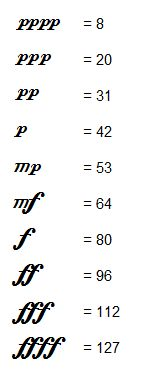
\includegraphics[width=0.1\textwidth]{imagens/nuance-velocity-table.jpg}
    \caption{Velocidades em notação musical e seus respectivos valores para a mensagem {\it Note On}}
  \label{fig:Velocidades em notação musical}
\end{figure}

Essa velocidade de reprodução, dependendo do tipo de instrumento selecionado, também varia a dinâmica que o som é reproduzido como quando uma nota de um piano é pressionada de forma brusca ou mais suave.
\begin{itemize}
  \item A mensagem {\it Note OFF}:
  \begin{itemize}
    \item {\it Status byte}: 1000 nnnn
    \item {\it Data byte}: 0kkk kkkk
    \item {\it Data byte}: 0vvv vvvv
  \end{itemize}
\end{itemize}

Para as mensagens {\it Note OFF}, os {\it bits} nnnn e kkkkkkk representam o mesmo da mensagem de ativação da nota sendo diferente apenas no terceiro {\it byte}, o vvvvvvv, que representa a velocidade de {\it release} do som, ou seja, a suavização até ele ser desligado.

A mensagem de alteração de valores dos controladores é representada da seguinte maneira:
\begin{itemize}
  \item A mensagem {\it Control Change}:
  \begin{itemize}
    \item {\it Status byte}: 1000 nnnn
    \item {\it Data byte}: 0ccc cccc
    \item {\it Data byte}: 0vvv vvvv
  \end{itemize}
\end{itemize}

Onde nnnn representa o canal para o qual a mensagem será enviada, da mesma forma das mensagens de ativação e desativação do som, ccccccc representa o controlador que terá o seu valor alterado e vvvvvvv representa o valor que será atribuído para o controlador. Os controladores controlados a partir dessas mensagens podem variar entre 128 controladores destintos sendo eles os seguintes:

FOTO DOS CONTROLADORES

Com essa mensagem, é possível variar, em cada canal, desde variáveis de volume, até variáveis de modulação e efeitos que caracterização como o som será reproduzido pelo sintetizador.

\chapter{Marcadores ArUco}
\label{cha:fund-teor}

A funcionalidade do software projetado nesta tese depende intrinsecamente da AOI ({\it area of interest}) do {\it layout} e, para se adquirir essa área de interesse da imagem inicial, uma das soluções mais comuns é a utilização de marcadores fiduciais quadrados binários. O principal benefício em se utilizar marcadores do tipo é de se obter, a partir dos quatro cantos de um único marcador, a {\it camera pose}, ou seja, tanto a orientação quanto a posição da câmera no ambiente.

No desenvolvimento deste projeto foi escolhido o módulo Aruco da biblioteca de visão artificial OpenCv para geração e identificação desses marcadores.O módulo Aruco é baseado na biblioteca ArUco, uma popular biblioteca utilizada para detecção de marcadores fiduciais quadrados, desenvolvida por Rafael Muñoz e Sergio Garrido, em aplicações de realidade aumentada.

A partir do módulo Aruco, pode-se gerar marcadores ArUco que consistem em marcadores quadrados compostos por uma larga borda da cor preta e uma matriz binária intríseca ao marcador, que determina seu identificador. As bordas existem para facilitar a detecção do marcador em uma imagem e a codificação da matriz binária para permitir a detecção desse marcador com intuíto de serem aplicadas outras técnicas de visão artifial. Abaixo temos alguns exemplos de marcadores ArUco:

IMAGEM MARCADORES ARUCO

Com uma detecção rápida e precisa desses marcadores, feita pela biblioteca OpenCv, foram escolhidos quatro identificadores que simbolizam os cantos da folha modelo e o software, ao decodificar os quatro marcadores, dependendo do seu identificador, são selecionados 4 pontos, um de cada marcador, a fim de adquirir a área de interesse da folha para o software.

IMAGEM DOS QUATRO PONTOS IDENTIFICADOS

Com a área de interesse adquirida, é aplicada uma transformação de perspectiva nessa nova imagem a fim de  desprezar distorções causadas pelo posicionamento da câmera, uma vez que esta nova imagem que será analizada pelo software precisa ser paralela à folha, o que é possível a partir de diferentes ângulos, isso se os quatro marcadores forem visíveis, graças a transformação de perspectiva, fazendo o usuário manusear o software de forma mais confortável.

Outra forma de identificação que foi testada no projeto foi por cores em círculos coloridos posicionados no canto da folha. Devido à diversas variáveis de ambiente, essas cores poderiam variar de usuário para usuário, local para local, câmera para câmera entre outros, o que tornava necessária a marcação das cores ser feita manualmente pelo usuário com o propósito de haver um cálculo da média da cores dos círculos para sua identificação e, devido a essa inconsistência ao utilizar cores, a ideia foi descartada. O modelo anterior pode ser visto abaixo:

IMAGEM DO MODELO COM OS CÍRCULOS


\chapter{Transformação de Perspectiva}
\label{cha:fund-teor}

Para o software interpretar a imagem de forma correta, é necessário que ela seja paralela à câmera, tornando desconfortável a sua utilização. Uma maneira de solucionar esse problema foi utilizar uma transformada de perspectiva, desprezando os problemas gerados para imagens capturadas de posições que não sejam paralelas à câmera que está capturando o ambiente.

Graças à biblioteca OpenCv, essa manipulação é de rápida e fácil aplicação, precisando-se apenas de quatro pontos de referência na imagem original e uma nova matriz imagem resultado.



Assuntos a serem abordados:
- Descrever a MATEMÁTICA envolvida nessa transformação 

\chapter{Como Utilizar o Software}
\label{cha:fund-teor}

Ao se iniciar o software, é necessário passar três parâmetros iniciais na sua execução. O primeiro é o identificador da entrada de vídeo do usuário para a cena ser capturada com a câmetra correta caso haja mais de uma conectada.

O segundo é a velocidade de batidas por minuto (bpm) para o tempo de referência para reprodução das notas reproduzidas pelo software. Ao gerar o modelo da folha, o usuário deve passar os valores que formarão a fórmula do compasso para aquela folha em específico, porém, devido à limitação de espaço de uma folha A4, não é possível utilizar qualquer fórmula de compasso que se deseja. Um exemplo que faria com que o software apresentasse inconsistência pode ser encontrado abaixo:

LAYOUT COM 4/16

Podemos ver que, dependendo do que o usuário definisse, a espaço livre para as marcações do usuário seria mínio, prejudicando o funcionamento do software.

O terceiro é a oitava que será reproduzida no software. A oitava, na teoria musical, representa uma nota com o dobro ou metade de sua frequência. É quando a nota será, apesar de ter uma frequência maior ou menor que a nota de referência, a mesma e se chama oitava devido ao fato de, na representação mais comum das notas (dó, ré, mi, fá, sol, lá, sí), ela seria a oitava nota, que seria a mesma da primeira porém com uma frequência dobrada, ou seja: dó (oitava x), ré, mí, fá, sol, lá, sí e dó (oitava x+1), onde o último só e a oitava nota em relação ao primeiro.

Com esses paramêtros definidos, o software inicia-se e lista todas as entradas midi disponíveis no momento para o usuário escolher a que o software enviará as mensagens do protocolo. Os parâmetros iniciais informados pelo usuário ao iniciar o software são apenas para configuraão inicial do ambiente, porém, ao iniciar-se o software de maneira correta, são editáveis a partir do clique de teclas específicas informadas pelo programa.

Após essas configurações iniciais, é preciso se cumprir, assim como outros softwares que utilizam conceitos de visão artificial, certas condições para o funcionamento correto do software projetado neste trabalho.
Primeiramente precisa-se de condições de ambiente favoráveis à captura das imagens da câmera como iluminação da cena, principalmente de forma que a folha não fique muito escura ou com sombreados escuros, pois o filtro de branco utilizado na área de interesse pode identificar essas sombras como marcações, o prejudica no funcionamento do software. Outra condição é uma angulação da câmera de forma que se consiga visualizar os quatro marcadores ArUco e o código de barras presentes na folha. Marcações serão mostradas no vídeo quando os cinco elementos forem identificados de forma correta. Abaixo temos a imagem capturada pela câmera com as devidas marcações indicando que as instruções iniciais foram seguidas como o desejado:

FOTO COM AS MARCAÇÕES DE QUE ESTÁ TUDO OK

A partir desse ponto, pode-se utilizar a barra de espaço para o software tocar ou parar a sequência identificada na folha. Essa sequência pode ser livremente alterada pelo usuário diretamente na folha de papel e reproduzida novamente quando se desejar, bastando apenas que as condições já explicadas sejam sempre cumpridas antes de se informar ao software que ele deverá reproduzir a sequência da folha.

As marcações devem ser feitas sempre o mais centralizadas possível no retângulo que indica o espaço de tempo da sequência, sendo possível representar sons que vão continuar soando ou que vão parar no próximo intervalo de tempo com duas marcações distintas já mostradas no capítulo que destrincha o algoritmo utilizado.

\chapter{Biblioteca RtMidi}

Como já visto no capítulo (capítulo do protocolo midi), o sintetizador escolhido pelo usuário precisa receber as mensagens enviadas pelo software e foi com auxílio da biblioteca RtMidi para a linguagem de programação C++ que foi possível abstrair todo o fluxo de troca de mensagens em simples funções disponibilizadas pela biblioteca.

Para a utilização do protocolo MIDI e para a comunicação entre sintetizadores, foi escolhida a biblioteca RtMidi para a linguagem de programação C++. Toda a transmissão e criação das mensagens foi abstraída durante o desenvolvimento do projeto graças às funcionalidades da biblioteca e foi por esse motivo, além de ser Open Source, que ela foi escolhida para fazer parte do desenvolvimento do software.

A biblioteca consiste em duas classes chamadas RtMidiOut e RtMidiIn. A classe RtMidiOut proporciona, para o desenvolvedor, funcionalidades simples para a imediata troca de mensagens MIDI entre dispositivos virtuais ou não conectados através de uma conexão MIDI. Com essas funcionalidades foi possível ocorrer o envio de mensagens para o sintetizador selecionado pelo usuário como porta de entrada ou cliente para escrita da conexão midi com apenas o uso, após configurada essa entrada, de uma função responsável exclusivamente pelo envio dessas mensagens. A outra classe, RtMidiIn, apesar de não ter sido utilizada no software apresentado neste trabalho, utiliza uma função interna de callback ou thread para receber mensagens MIDI que são enviadas a partir de uma porta de saída MIDI selecionável e as lendo, transformando no formato utilizado pela biblioteca, ou repassando-a imediatamente para uma função de callback especificada pelo usuário, o que tornaria possível, por exemplo, o software reproduzir, num sintetizador digital, o que foi enviado a partir de um controlador físico conectado à máquina do usuário.

Para o testes do software, foram utilizados 3 softwares de terceiros, sendo eles o QSynth, sintetizador virtual MIDI, o VMPK, outro sintetizador virtual MIDI mas também controlador, e o QJackCtl, um software que permite o usuário administrar as conexões MIDI entre saídas e entradas MIDI disponíveis na máquina.
TUDO ABAIXO SERÁ EXPLICADO NESTE ÚTIMO CAPÍTULO

- Descrever o sintetizador usado nos experimentos (QSynth).


- Descrever como se dá, no Linux, a interligação entre seu software
Controlador e o Sintetizador. Um diagrama legal feito no inkscape
cairia bem nesse canto.
O diagrama a seguir representa como o software controlador se comunica com um sintetizador
DIAGRAMA (MIDI INPUT, OUPUT, SOFTWARE CONTROLADOR E SINTETIZADOR)
BASICAMENTE SOFTWARE (CONTROLADOR) COMO OUTPUT LIGADO NO SINTETIZADOR (VMPK OU QSYNTH) COMO INPUT E A TROCA DE MENSAGENS OCORRE DO CONTROLADOR PARA O SINTETIZADOR.

\chapter{Resultados}
\label{cha:resultados}

Apresentar exemplos de uso da ferramenta...

Tem um software bem legal de composição chamado rosegarden. Ele também
funciona como um ``sintetizador m MIDI'', pois aceita entradas do
controlador para permitir composições. Prepare um loop de exemplo e
conecte a saida do seu controlador na entrada do rosegarden. Observe a
sequencia gerada no software. Salve a sequencia e verifique se é
possível, usando o rosegarden, repetir a sequencia de loops conectando
agora rosegarden->qsynth.

Se funcionar legal (acredito que funcionará sem problemas), terás um
resultado muito bom, pois poderá mixar várias combinações possíveis
usando o rosegarden.

\chapter{Conclusões}
\label{cha:conclusoes}

Revise em linhas gerais o algoritmo desenvolvido e mostre os
progressos que obteve, comentando resultados e dificuldades
enfrentadas.

Proponha melhorias para a sua criação.

\bibliography{referencias}

\end{document}
